\vspace{-5pt} 
\section{Simulations}\label{sec:sims}

This section presents the simulation results for corroborating the performance of the proposed algorithms in diverse settings.

\vspace{-5pt} 
\subsection{Settings}

The simulations are based on a microgrid setting with a number of customers, each having a power demand and valuation generated according to a probability preference model. The customers may suffer from a reduction of generation capacity occasionally. The appearances and levels of reduction vary according to a stochastic process model.  

The model is designed to resemble  a real-world scenario, where the microgrid has a total capacity $C$ up to 2MVA connecting to residential customers (with relatively small demand) and industrial customers (with considerably large demand).

The algorithms ({\sc GVA}, {\sc GDA}, {\sc GRA}, {\sc 1DPA}) are applied to both valuation-maximizing and compensation-minimizing problems. 
The simulations were evaluated using 2 Quad core Intel Xeon CPU E5520s 2.21 GHz processors. The algorithms were implemented using C and Python programming languages and a standard random number generation library.
Each customer's reactive power demand equals to $ Q_k = \tan (\phi) \cdot P_k $, where $\phi$ is the phase angle between the reactive and apparent powers. %, and $\phi \in [0, 36]$ according to Electrical Power Engineering standards \cite{citation02}.

\vspace{-5pt} 
\subsection{Scenarios}

Diverse scenarios are considered in the following aspects.

\noindent
i) Power demands:
\begin{enumerate}

\item {\em Full (F) power}: The power demand of each customer can have both non-negative active power ($P_k \ge 0$) and non-negative reactive power ($Q_k \ge 0$).

\item {\em Active (A) power only}: The power demand of each customer can have non-negative active power ($P_k \ge 0$) but zero reactive power ($Q_k = 0$).

\end{enumerate}

\noindent
ii) Valuation/Compensation-demand correlation:
\begin{enumerate}

\item {\em Correlated (C)}: The valuation/compensation of each customer is a function of the power demand:
\begin{equation}\label{eq:valuationfunction}
u_k({|S_k|}) = a({|S_k|})^2 + b{|S_k|} + c 
\end{equation}
where $a > 0, b, c \ge 0$ are constants.

\item {\em Uncorrelated (U)}: The valuation/compensation of each customer is independent of the power demand and is generated randomly from $[0, a({|S_k|})^2 + b{|S_k|} + c]$.

\end{enumerate}

\noindent
iii) Customer types
\begin{enumerate}

\item {\em Industrial (I) customers}: Customers have big active power demands ranging from 300KW up to 1MW.

\item {\em Residential (R) customers}: Customers have small active power demands ranging from 500W to 5KW.

\item {\em Mixed (M) customers}: Customers have a mix of both industrial and residential customers

\end{enumerate}
In the following, a scenario is represented by the acronyms of the types. For example, scenario ACI stands for the one with industrial customers, zero reactive power demands and valuations/compensations-demand correlation.\\

\iffalse
{\em Valuation Model:} 

When the customer's valuation/compensation $u_k$ is correlated with its demand, it is calculated using the valuation function $u_k(|S_k|)$, which indicates the cost of consuming $S_k$ units of energy. We make the following assumptions:\\

\begin{enumerate}

\item
The valuation function is increasing based on the
consumed energy capacity. In other words, for each $k \in {\cal N}$, we have
\begin{center}
${u_k}({|S_k|}) \le {u_k}({{|S'_k|}}), \forall$   $ {|S_k|} \le {{|S'_k|}}$
\end{center}


\item The valuation function is strictly convex. For each  $k \in {\cal N} $, any $0 \le \alpha \le 1$, and ${|S_k|},{|S'_k|} \ge 0$, we have
\begin{center}
$u_k(\alpha |S_k| + (1 - \alpha)|S'_k|) \le \alpha u_k(|S_k|) + (1 - \alpha)u_k(|S'_k|)$
\end{center}
\end{enumerate}
\vspace{3mm}
Among various valuation functions that satisfy the aforementioned assumptions in this paper we use the following quadratic valuation function 
\begin{equation}
\label{eq:valuationfunction}
u_k({|S_k|}) = a({|S_k|})^2 + b{|S_k|} + c 
\end{equation}
where $a > 0, b, c \ge 0$ are pre-determined constants.\\

\fi


\vspace{-5pt}
\subsection{Results}


%In general, {\sc 1DPA}'s performance, in terms of the running time and maximized valuation, varies for different input values of $\epsilon$, that is the higher the $\epsilon$ the higher the running time and the lower the maximized valuation and vice versa. In our simulations the $\epsilon$ value for {\sc 1DPA} algorithm  was set to $10^{-18}$ in order to have as accurate results as possible but keep the running time up to 3 minutes. 

A summary of the simulation results for each the scenario is shown in Table \ref{algorithmscomparison}, which indicate most superior algorithm in the respective scenario. Specifically, fours scenarios are highlighted in Figs.~\ref{fig:scenarioaurfcm}-\ref{fig:scenariofuracm}

\begin{table}[h]
\renewcommand{\arraystretch}{2}
\centering \vspace{-5pt}
\begin{tabular}{lc|l|l|l|l|}
\cline{3-6}
 & \multicolumn{1}{l|}{} & \multicolumn{2}{c|}{F} & \multicolumn{2}{c|}{A} \\ \hhline{~~|-|-|-|-|} %\cline{3-6} 
 & \multicolumn{1}{l|}{} & \multicolumn{1}{c|}{C} & \multicolumn{1}{c|}{U} & \multicolumn{1}{c|}{C} & \multicolumn{1}{c|}{U} \\ \hline
\multicolumn{1}{|c|}{\multirow{2}{*}{{\sc maxPA}}} & R & GRA & GRA & \cellcolor[gray]{.8} 1DPA & \cellcolor[gray]{.8} 1DPA \\ \hhline{|~|-|-|-|-|-|} % \cline{2-6} 
\multicolumn{1}{|c|}{} & M & GDA & \cellcolor[gray]{.8}1DPA &\cellcolor[gray]{.8} 1DPA &\cellcolor[gray]{.8}  1DPA \\ \hline
\multicolumn{1}{|l|}{\multirow{2}{*}{\sc minPA}} & R & GRA & GRA & \cellcolor[gray]{.8} 1DPA &\cellcolor[gray]{.8}  1DPA \\ \hhline{|~|-|-|-|-|-|}% \cline{2-6} 
\multicolumn{1}{|l|}{} & M & GDA & \cellcolor[gray]{.8}  1DPA & \cellcolor[gray]{.8} 1DPA & \cellcolor[gray]{.8}  1DPA \\ \hline
\end{tabular} \vspace{-5pt}
\caption{The results of simulations in each scenario. Each cell of the table indicates the most superior algorithm in the respective scenario.}
\label{algorithmscomparison}
\end{table}

\vspace{-5pt}
\subsubsection{Empirical Ratios with Optimal Solutions}~\\

\begin{figure}[!htb]\vspace{-5pt}
	\begin{center}
		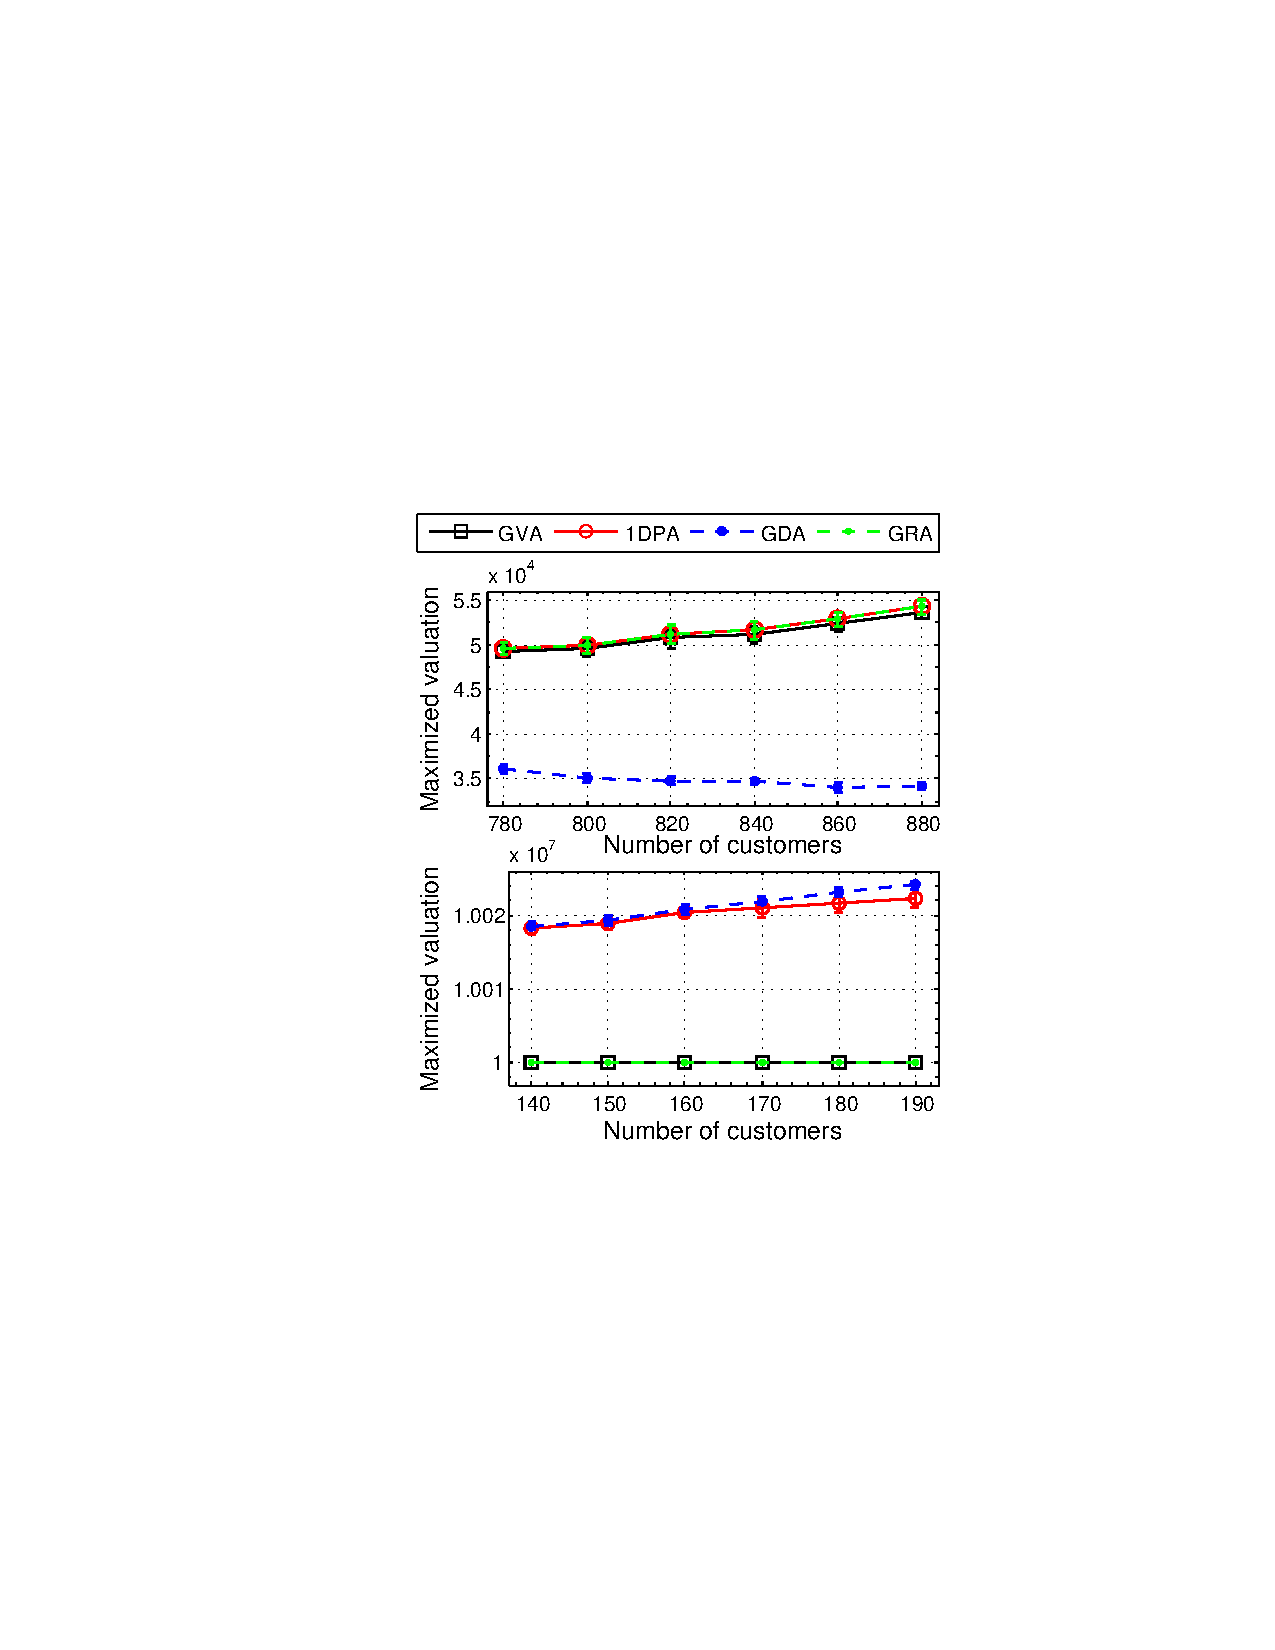
\includegraphics[scale=0.7]{fig/4_5.pdf}
	\end{center}\vspace{-5pt}
\caption{{\sc GVA}, {\sc GDA}, {\sc GRA}, {\sc 1DPA} apply to {\sc maxPA} for scenarios AUR and FCM on top and bottom respectively.}
	\label{fig:scenarioaurfcm}
\end{figure} 

 When customers' reactive demand $Q_k$ is not taken into account, {\sc maxPA} and {\sc minPA} for {\sc 1DPA}  become a simple classical knapsack problem. In fact, in that case the maximized valuation and minimized compensation by {\sc 1DPA} is considerably close to the possible optimal value. This can be seen from Fig.~\ref{fig:scenarioaurfcm} and Table \ref{algorithmscomparison}, which show that {\sc 1DPA} algorithm outperforms all greedy algorithms mentioned in this paper.\\

On the other hand, when customers' reactive demand is considered,  {\sc maxPA} and {\sc minPA} become computationally complex problems for {\sc 1DPA}. In this case {\sc GVA}, {\sc GDA}, {\sc GRA}, and {\sc 1DPA}'s performance varies for these cases when the customers are only residential and when there is a mix of residential and industrial customers as indicated in Fig.~\ref{fig:scenariofuracm} and Table \ref{algorithmscomparison}.

To sum up, the aforementioned simulations show that two key factors, namely the correlation between valuation/compensation and demand, and customers' apparent power, have a substantial impact on the performance of {\sc GVA}, {\sc GDA}, {\sc GRA}, and {\sc 1DPA}.

\begin{figure}[!htb]\vspace{-5pt}
	\begin{center}
		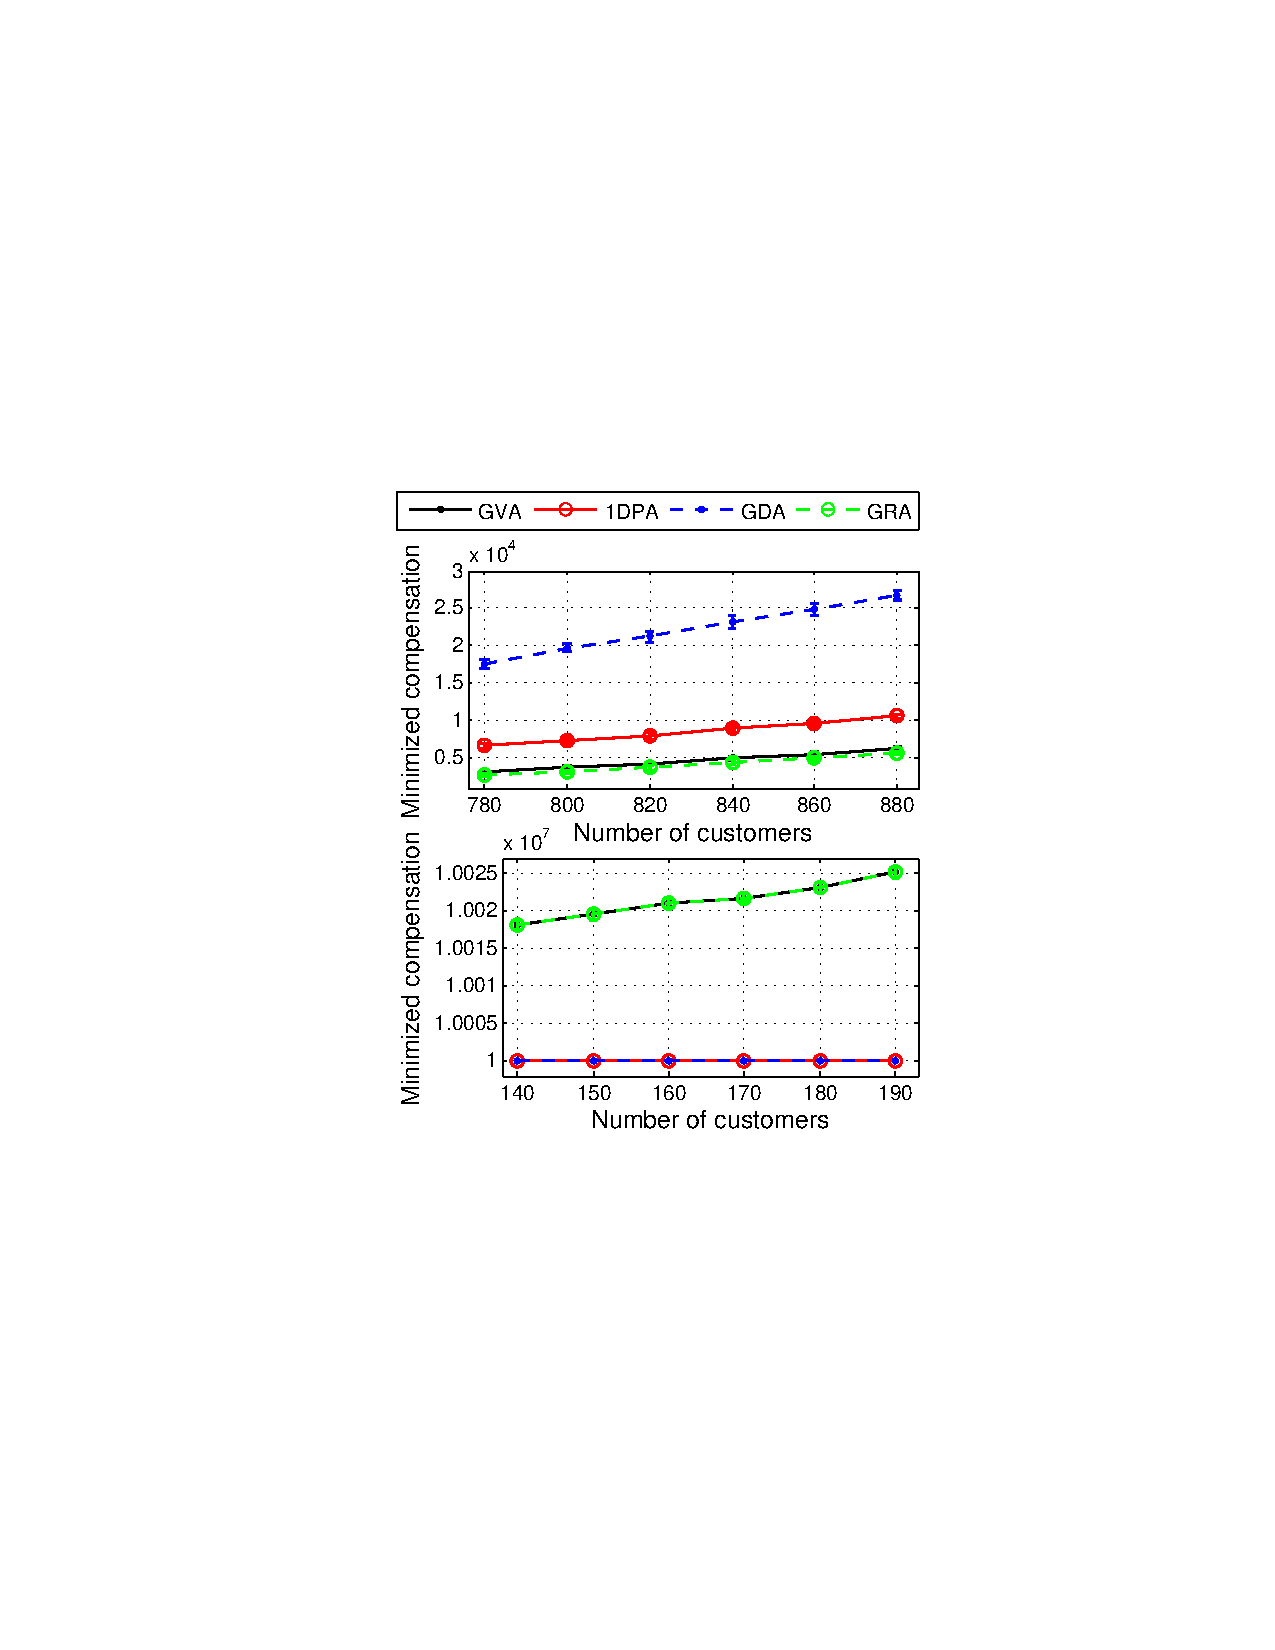
\includegraphics[scale=0.7]{fig/1_8.pdf}
	\end{center}\vspace{-5pt}
\caption{{\sc GVA}, {\sc GDA}, {\sc GRA}, {\sc 1DPA} apply to {\sc minPA} for scenarios FUR and ACM on top and bottom respectively.}
	\label{fig:scenariofuracm}
\end{figure} 

The importance of the load (i.e.,  the priority and the benefit to the system) are among various fundamental factors that should be carefully considered when planning a load curtailment algorithm \cite{466502}. The conventional load curtailment strategies used in power grids (i.e., curtailing loads simply according to the ascending order of priorities \cite{5348255,6493097}), are basically {\sc GVA}, when valuations reflect the priorities.

For the case when the microgrid customers have strictly defined priorities and customers with high priorities are of critical importance and should never be curtailed, the {\sc GVA} is an effective algorithm. Nevertheless, the analysis of the results shows that when the loads have the same or no priority like that in the simulations, in such cases the {\sc GVA} does not produce high valuation or low compensation cost solutions, which can be seen in Table \ref{algorithmscomparison}.\\

 \vspace{-5pt}
\subsubsection{Running Time}
\hspace{2cm}
\begin{figure}[!htb]\vspace{-5pt}
	\begin{center}
		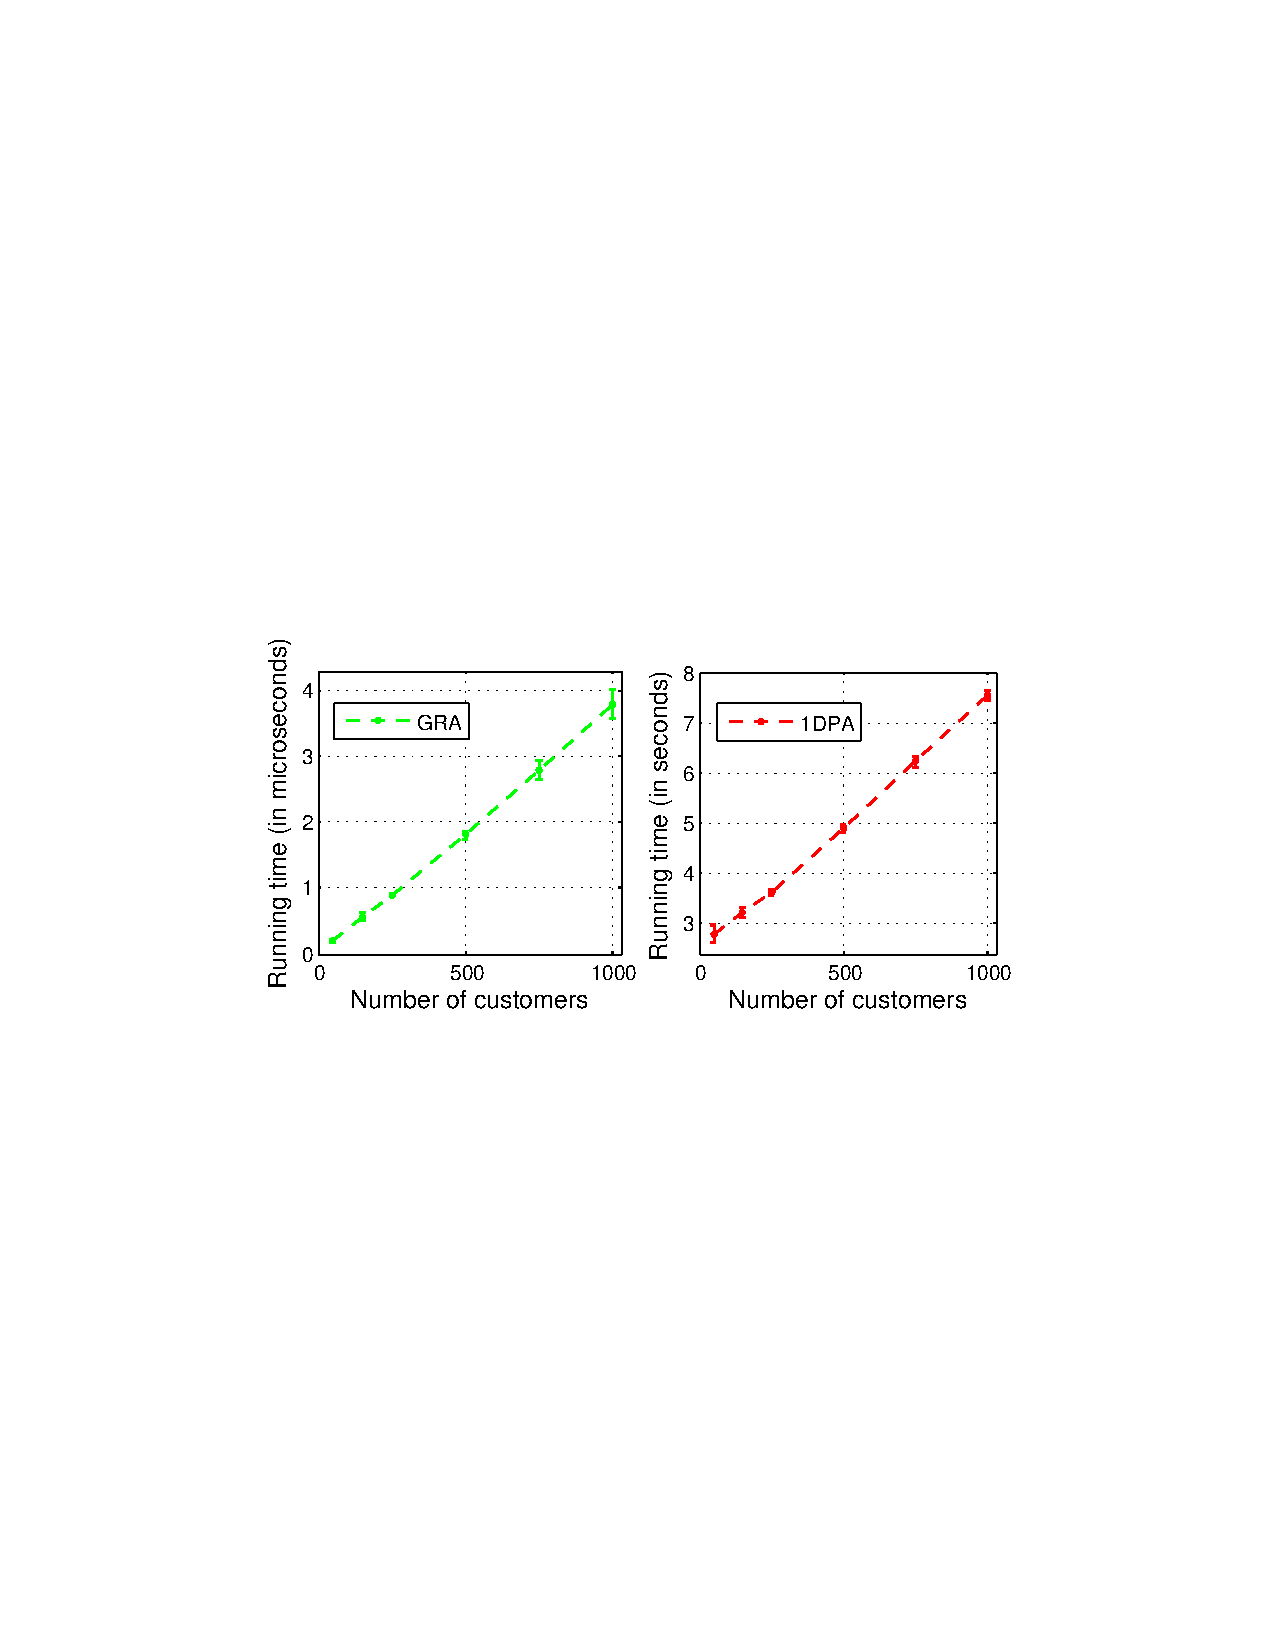
\includegraphics[scale=0.55]{fig/rt.pdf}
	\end{center}\vspace{-5pt}
\caption{The running time of {\sc 1DPA} and {\sc GRA}.}
	\label{fig:rt}
\end{figure}



\begin{figure}[!htb]\vspace{-5pt}
	\begin{center}
		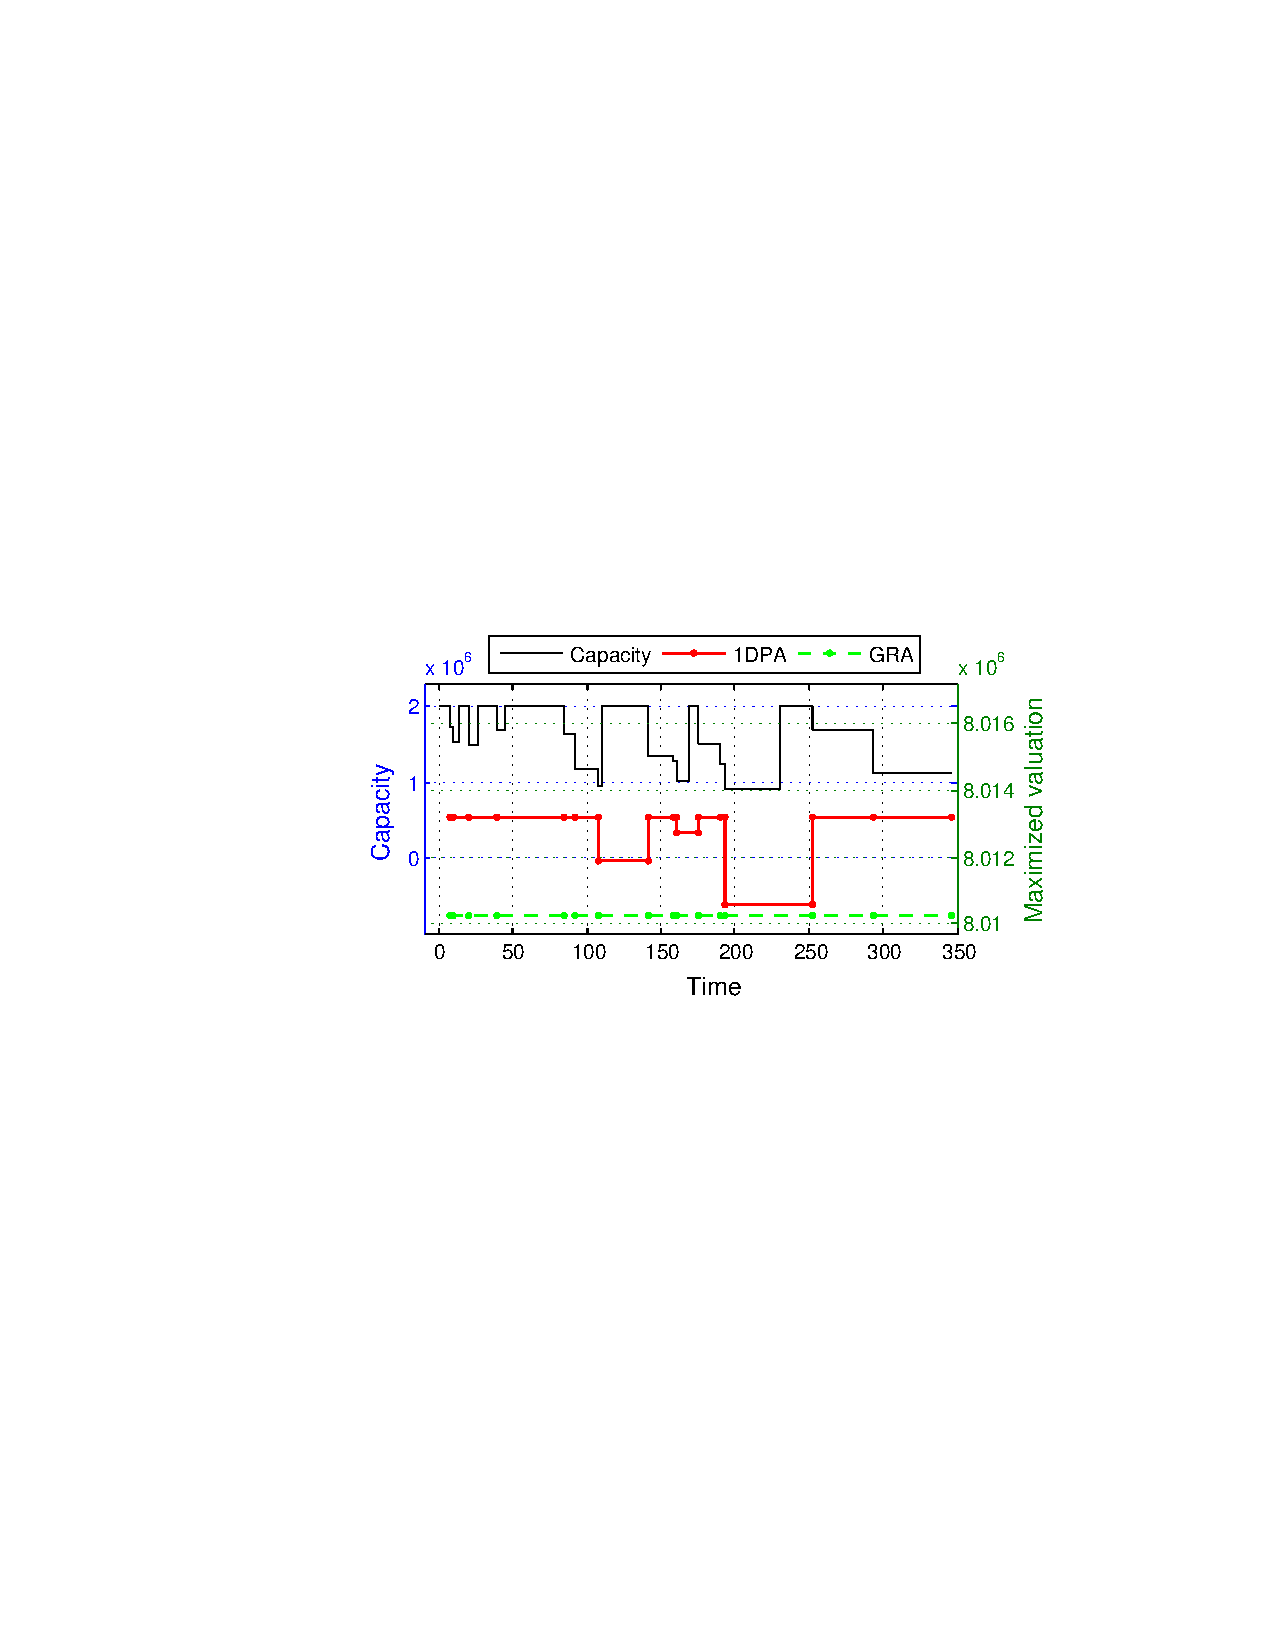
\includegraphics[scale=0.6]{fig/maxPa.pdf}
	\end{center}\vspace{-5pt}
\caption{{\sc 1DPA} and {\sc GRA} apply to {\sc maxPA} without power-off protection constraint for Scenario AUM.}
	\label{fig:maxpa}
\end{figure}

\begin{figure}[!htb]\vspace{-5pt}
	\begin{center}
		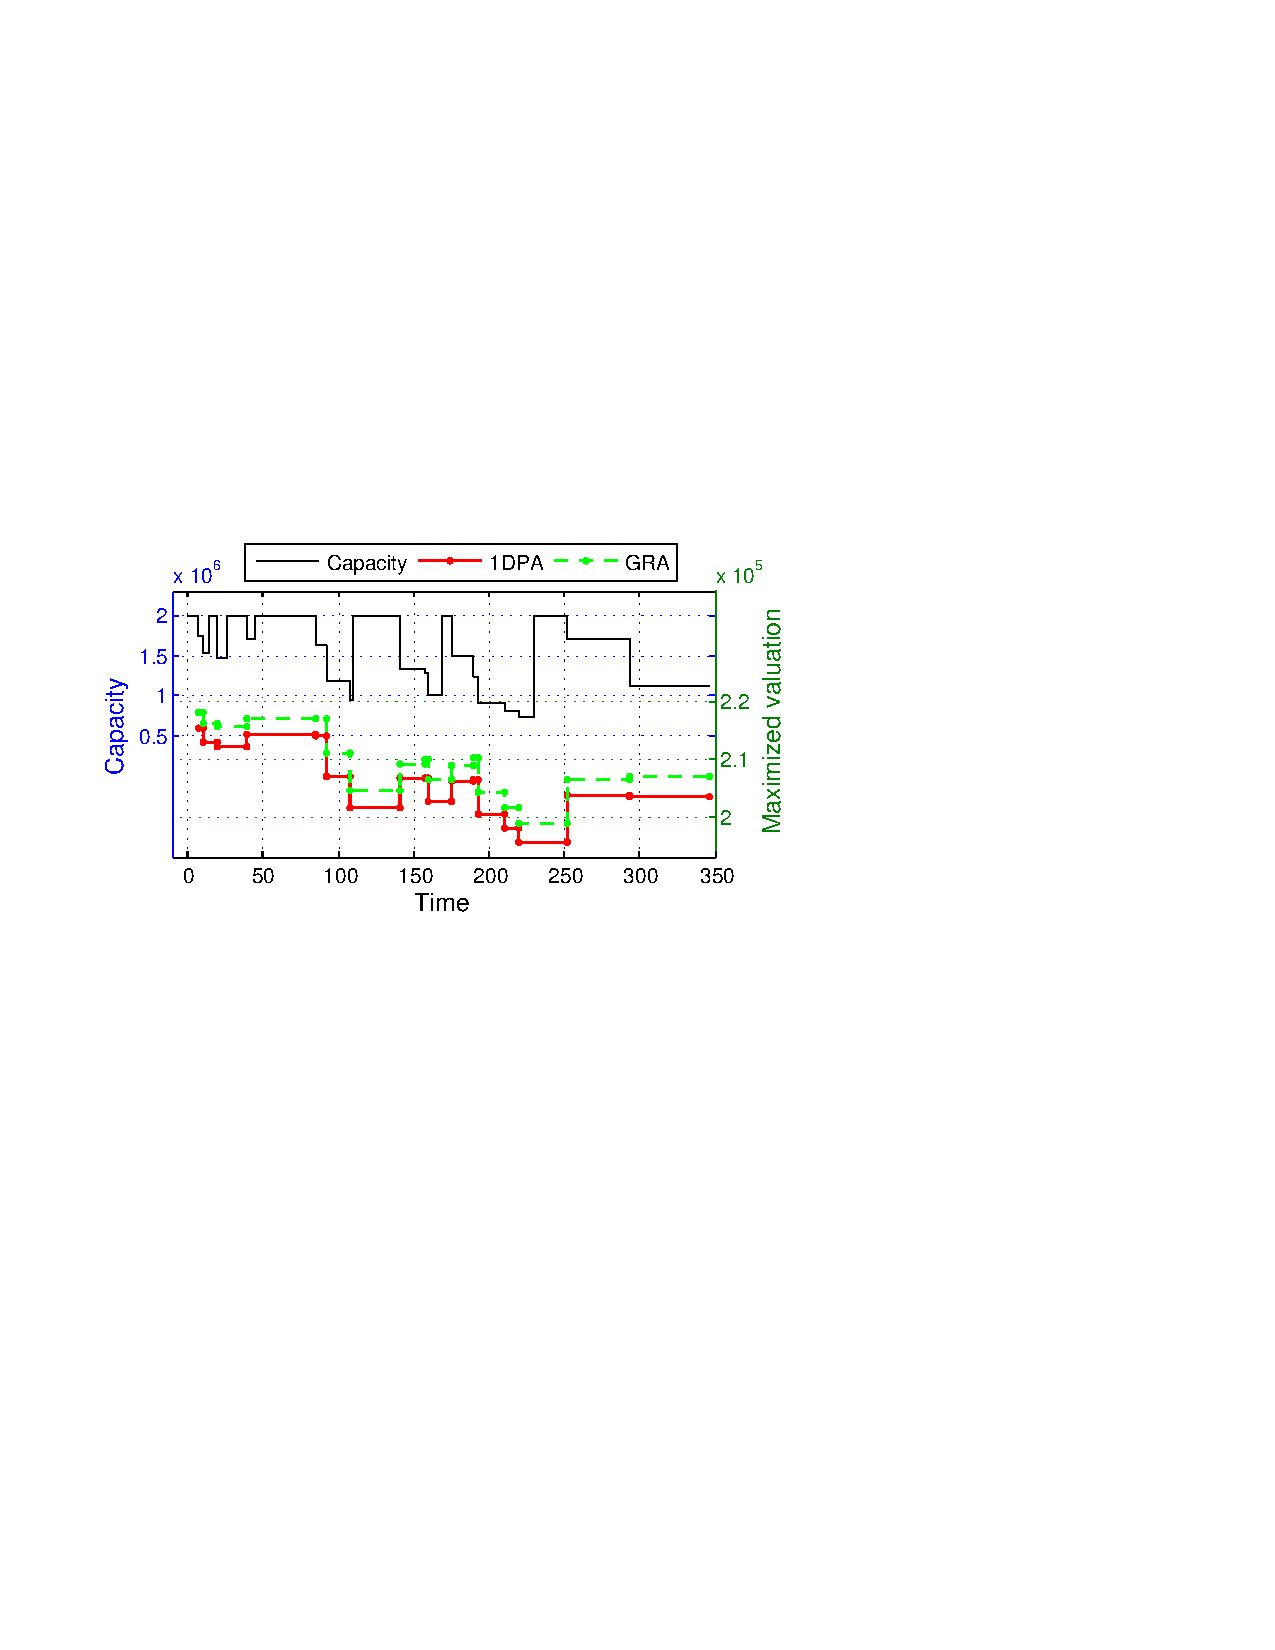
\includegraphics[scale=0.6]{fig/maxpatac.pdf}
	\end{center}\vspace{-5pt}
\caption{{\sc 1DPA} and {\sc GRA} apply to {\sc maxPA} with power-off protection constraint for Scenario FUR.}
	\label{fig:maxpatac}
\end{figure}

%\vspace{2mm}
One of the major parameters that evaluates an event-based demand response management algorithm is its running time. The algorithm should be sufficiently fast. Despite a considerable body of literature on this topic, however, they only considered microgrids with a significantly small number of customers, as compared to the number of customers considered in this paper. The running time with respect to a large number of customers is not studied.

Although in most cases {\sc 1DPA}'s solutions are remarkably close to the optimal, the running time is more than that of {\sc GRA}, especially in the scenarios with mixed customers. Generally, the more the number of customers, the larger is the running time, as seen from Fig.~\ref{fig:rt}.

Therefore, this paper proposes a two-stage hybrid approach to take advantage of both {\sc 1DPA} and {\sc GRA}.
\begin{figure}[!htb]
	\begin{center}
		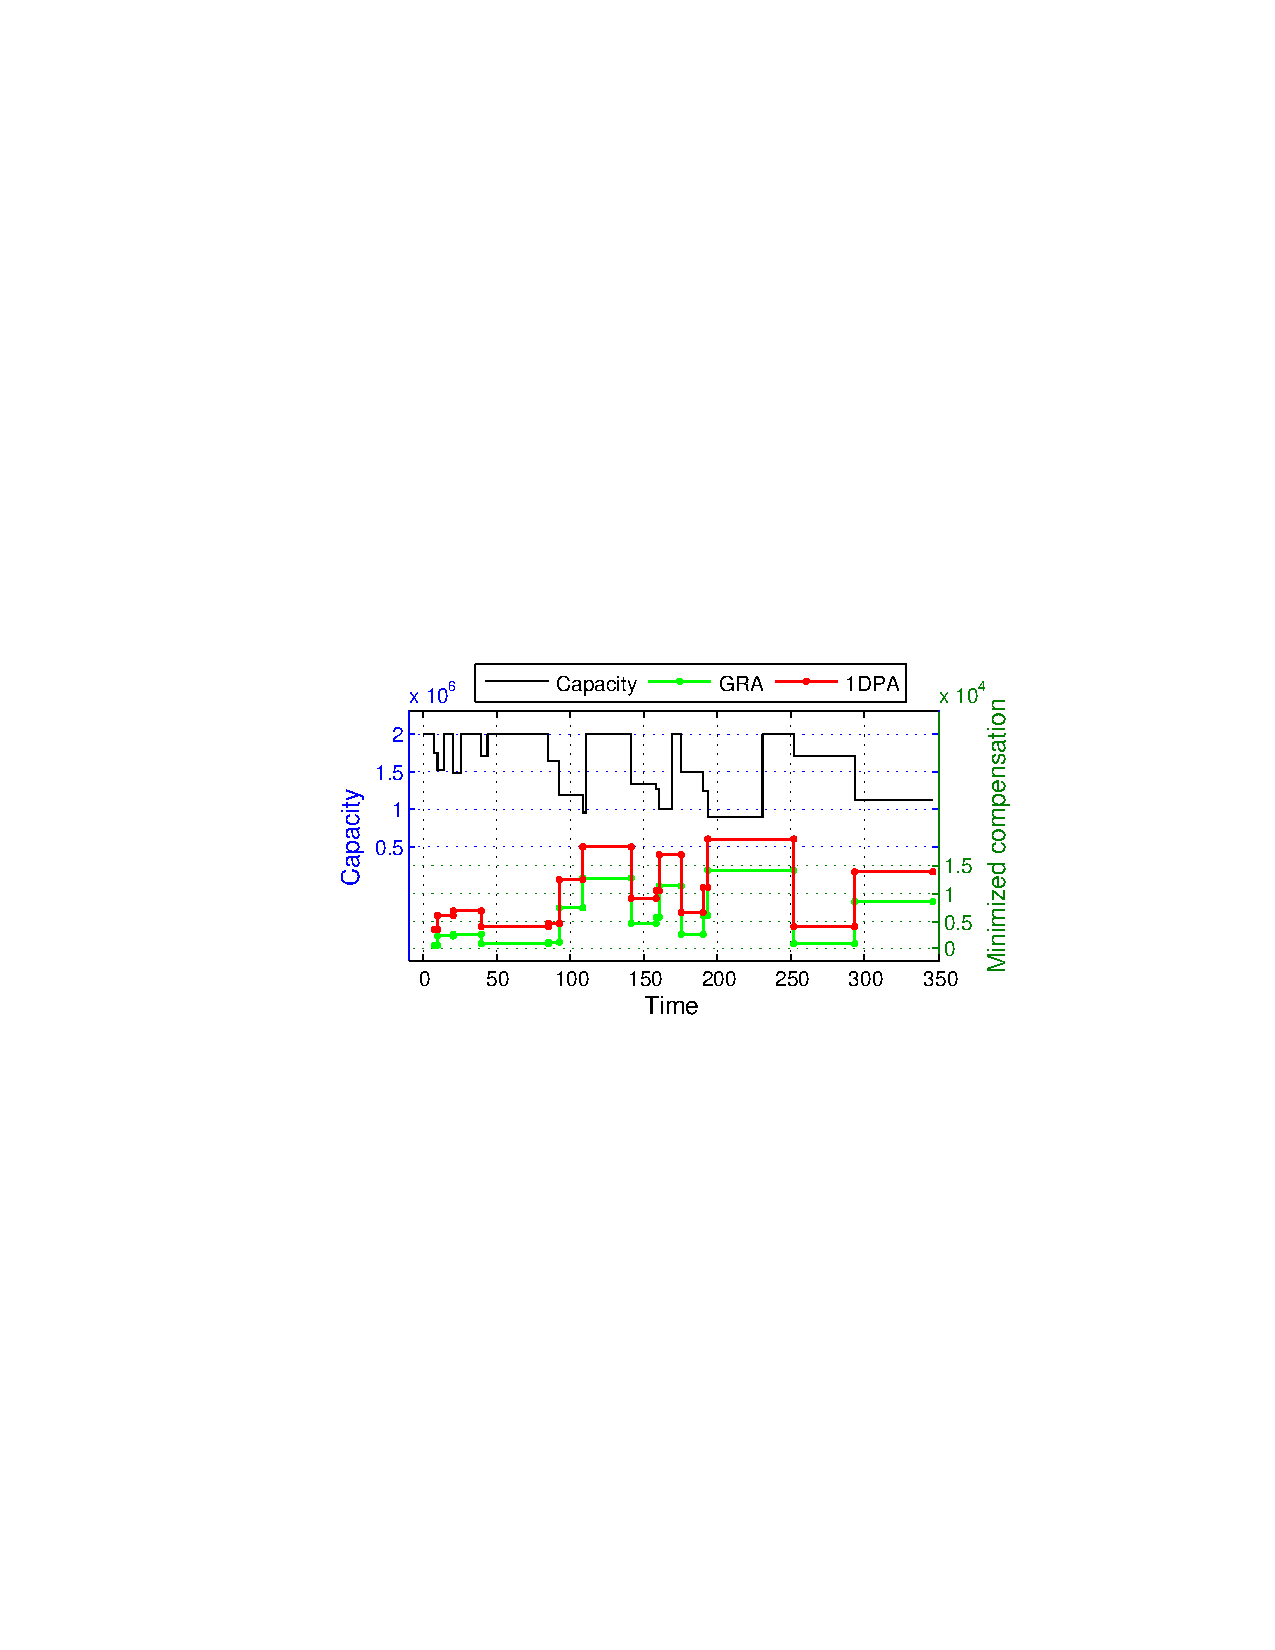
\includegraphics[scale=0.6]{fig/minpaac.pdf}
	\end{center}\vspace{-5pt}
\caption{{\sc 1DPA} and {\sc GRA} apply to {\sc minPA} without power-off protection constraint for Scenario FUR.}
	\label{fig:minpaac}
\end{figure}

\begin{figure}[!htb]\vspace{-5pt}
	\begin{center}
		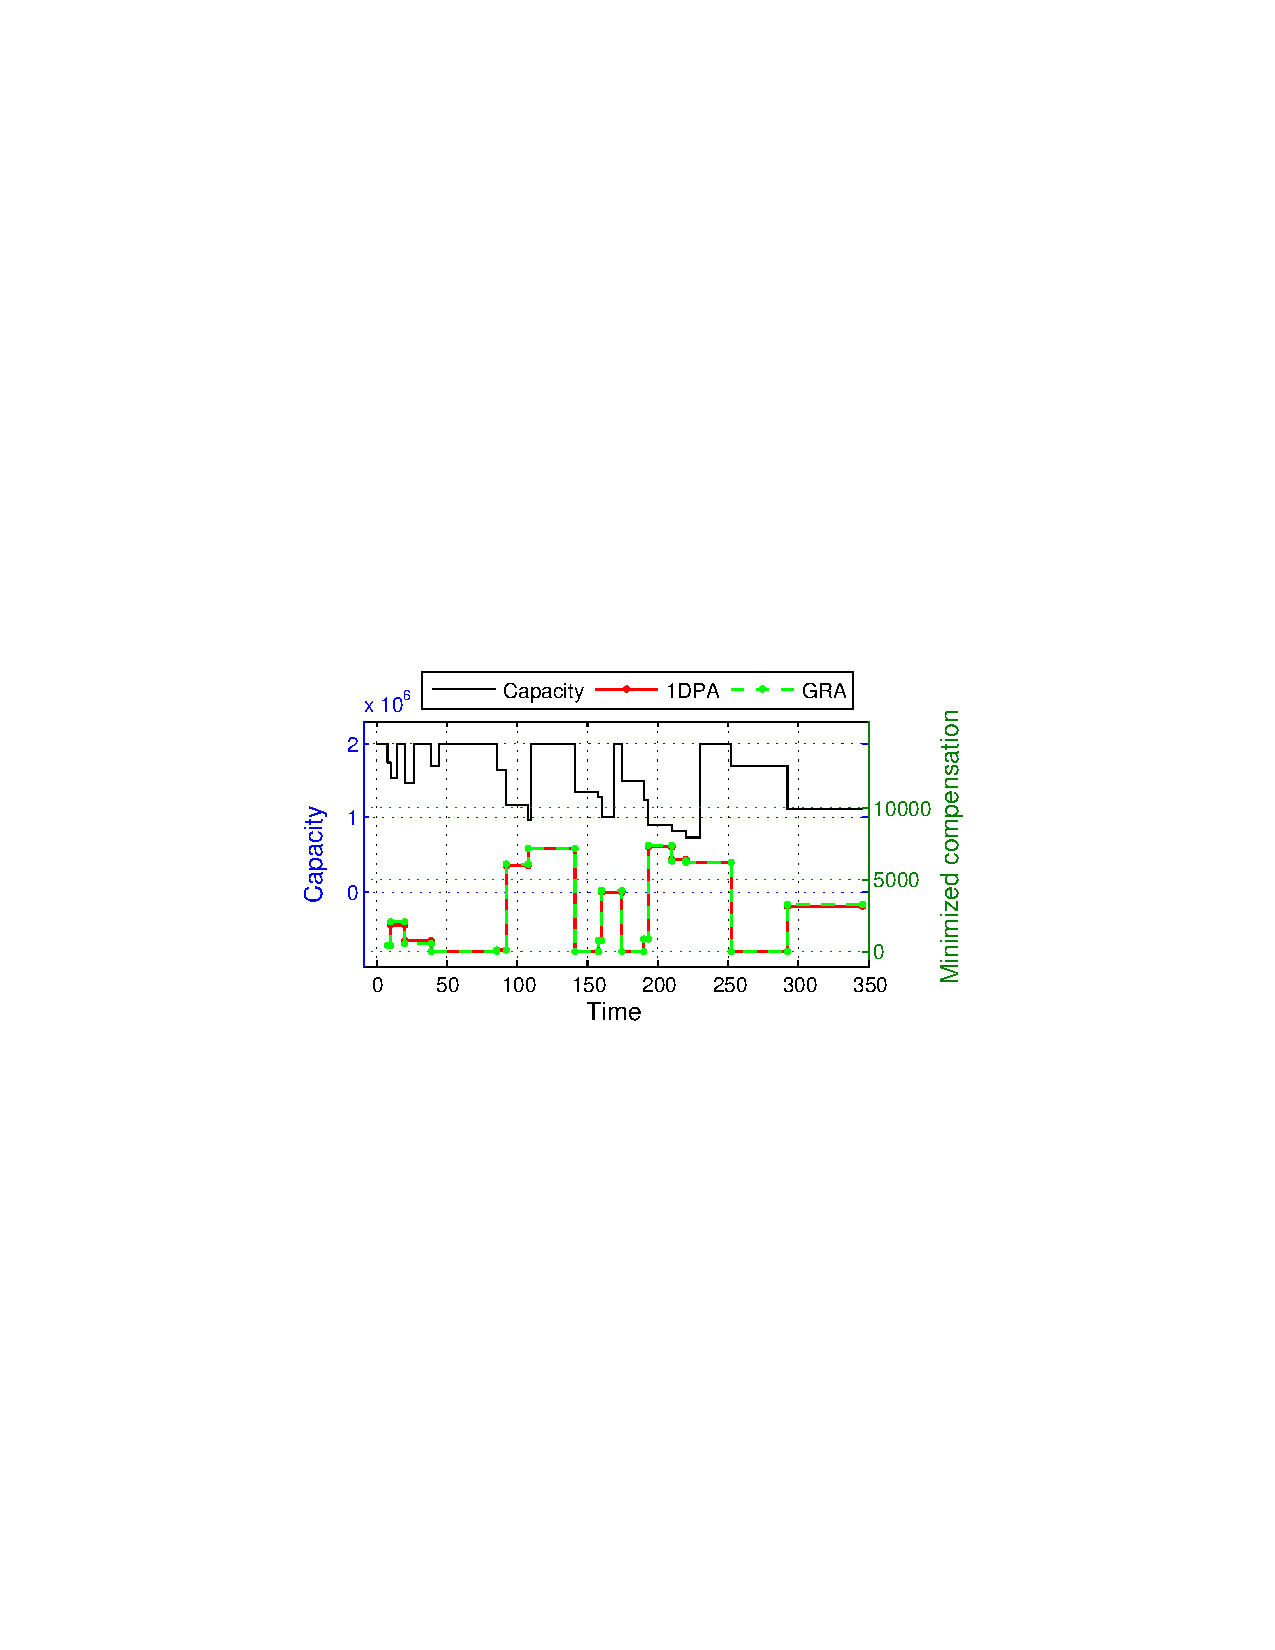
\includegraphics[scale=0.6]{fig/minpatdc.pdf}
	\end{center}\vspace{-5pt}
\caption{{\sc 1DPA} and {\sc GRA} apply to {\sc minPA} with power-off protection constraint for Scenario AUR.}
	\label{fig:minpatdc}
\end{figure}

 \vspace{-5pt}
\subsubsection{Dynamic Capacity}~\\


In addition to the aforementioned scenarios, simulations are performed considering the case when the microgrid's capacity is varying over time due to possible events (e.g., failure, or resumption), whereas the set of customers is fixed. 

The aforementioned scenario is applied to both {\sc maxPA} and {\sc minPA}  with and without power-off protection constraint. The events, namely Failure and Resumption, occur according to an exponential distribution with a n expected rate $200$. When the microgrid is in the Failure state, the capacity decreases randomly from $5\%-35\%$, whereas when in the Resumption state the microgrid's capacity is fully resumed (i.e.,  $C=$2MVA), except the times when an events occurred the remaining time the microgrid is in the Steady state (i.e., it remains at the same state as was in the previous). Whether an event is the Failure or Resumption state is determined according to a Markov chain with the following settings:
 \begin{enumerate}
 \item Steady $\rightarrow$ Failure with a probability of $65\%$
 \item Steady $\rightarrow$ Resumption with a probability of $35\%$
 \end{enumerate}
 
The value of $T^{\rm off}_k$ for each customer is generated randomly from a range $[0, |S_k| ]$. The results show that without power-off protection constraint for the scenarios with active power only, {\sc 1DPA} outperforms {\sc GRA} for both {\sc maxPA} and {\sc minPA}. In Fig.~\ref{fig:maxpa}, {\sc GRA}'s maximized valuation is lower than the one of {\sc 1DPA} and is constant. This is because {\sc GRA} simply fails to consider all the residential customers with small power demands as well as the remaining industrial customers whose power demand is relatively smaller compared to the industrial customers having considerably big power demand. For the other scenarios performance of {\sc 1DPA} and {\sc GRA} varies considerably based on the values of $T^{\rm off}_k$ as well as on customers' power demands' range, as seen from Figs.~\ref{fig:maxpatac},\ref{fig:minpaac},\ref{fig:minpatdc}.
